%% pfgguide.dtx Copyright (c) 1995 Michael C. Grant and Craig Barratt
%%              All rights are reserved.
%%
%%            This system is distributed in the hope that it will be
%%            useful, but WITHOUT ANY WARRANTY; without even the
%%            implied warranty of MERCHANTABILITY or FITNESS FOR A
%%            PARTICULAR PURPOSE. Don't come complaining to us if you
%%            modify this file and it doesn't work! If this file is
%%            modified by anyone but the authors, those changes and
%%            their authors must be explicitly stated HERE.
%%
\documentclass[11pt]{ltxguide}
\usepackage{shortvrb,psfrag,graphicx}

% I prefer more to a page.
\marginparsep 0pt \oddsidemargin 0pt \evensidemargin 0pt
\textwidth \paperwidth \advance \textwidth by-2in
\topmargin 0pt \headheight 0pt \headsep 0pt
\textheight \paperheight \advance \textheight by-2in

\let\pkg\textsf
\let\fname\texttt
\let\pscom\texttt
\newcommand{\pfg}{\pkg{PSfrag}}
\newcommand{\ie}{\emph{i.e.\@}}
\newcommand{\eg}{\emph{e.g.\@}}
\newcommand{\etc}{\emph{etc.\@}}
\newcommand{\netaddress}[1]{\texttt{#1}}
\MakeShortVerb{\|}
\def\cs#1{%
  {\ttfamily\expandafter\string\csname #1\endcsname}}
\providecommand\marg[1]{%
  {\ttfamily\char`\{}{\em#1\/}{\ttfamily\char`\}}}
\providecommand\oarg[1]{%
  {\ttfamily[}{\em #1\/}{\ttfamily]}}
\providecommand\parg[1]{%
  {\ttfamily(}{\em #1\/}{\ttfamily)}}

\title{The \pfg\ system, version 3}
\author{Michael C. Grant and David Carlisle\\
        \netaddress{psfrag@rascals.stanford.edu}}
\date{11 April 1998}

\begin{document}

\maketitle
\tableofcontents

\section{What is \pfg?}

Many drawing and graphing packages produce output in the Encapsulated
PostScript (EPS) format, but few can easily produce the equations and other
scientific text of which \TeX\ is so capable. On the other hand, many
\LaTeX\-based drawing packages are not as expressive or easy-to-use as these
stand-alone tools.

\pfg\ provides the best of both worlds by allowing the user to precisely
overlay Encapsulated PostScript (EPS) files with arbitrary \LaTeX\
constructions. In order to accomplish this, the user places a simple text
``tag'' in the graphics file, as a ``position marker'' of sorts. Then, using
simple \LaTeX\ commands, the user instructs \pfg\ to remove that tag from the
figure, and replace it with a properly sized, aligned, and rotated \LaTeX\
equation. \pfg\ also allows the user to place \LaTeX\ constructs directly into
the EPS file itself.

Dr.\ Craig Barratt wrote the original version of \pfg\ as a graduate student at
Stanford University. The interface has changed very little since then, but the
internals have been completely re-written. The current version of PSfrag is
maintained by Michael Grant and David Carlisle. Many thanks go to the members
of the \pfg\ mailing list, and to everyone who has submitted a bug report or
suggestion.

\section{\pfg\ necessities}

In order to use \pfg, you will need the following tools:
\begin{itemize}
\item A recent version of \LaTeXe\ and the \pkg{graphics} package.
	  \pfg\ currently requires the 1995/12/01 version or later of these
	  packages, but it is always best to have the most recent release.
\item If you wish to use the \pkg{seminar} package with \pfg, you
	  should make sure you have the 1997/10/13 version or later (see
	  section \ref{sec:sem-bug}).
\item A compatible DVI-to-PostScript driver (see below). \pkg{dvips} is
	  the primary choice of the \pfg\ developers, and is certainly the
 	  most widely-used.
\end{itemize}

The latest versions of \LaTeXe, the \pkg{graphics} package, \pfg,
and \pkg{dvips} can all be found on CTAN, the
Comprehensive \TeX\ Archive Network. The CTAN cites, and their mirrors,
include:
\begin{center}
  \begin{tabular}{lll}
    Name & IP address & Location \\ \hline
    |ftp.dante.de| & 129.206.100.192 & Germany \\
    |ftp.tex.ac.uk| & 128.232.1.87 & England \\
    |ftp.cdrom.com| & 165.113.58.253 & USA \\
  \end{tabular}
\end{center}

\subsection{Choosing a PostScript driver}
\label{sec:compat}

\pfg\ relies on some sensitive PostScript tricks to accomplish its goals. Due
to limited time and resources, the authors could not confirm that \pfg\ works
properly on every available PostScript driver. We have attempted to insure that
it will \emph{eventually} work on every driver that is fully comaptible with
the \pkg{graphics} package (\ie, one for which a \fname{.def} file is
provided.)

The drivers which have been confirmed to work with \pfg\ are:
\begin{center}
\begin{tabular}{lll}
Driver & Tested by & Compatibility \\ \hline
Thomas Rokicki's \pkg{dvips} & the authors &
fully compatible \\
Y\&Y's \pkg{DVIPSONE} & the authors &
fully compatible
\end{tabular}
\end{center}
Please help us add entries to this list! If \pfg\ works with your driver,
please let us know, so we can add it to the list. If possible, test your \pfg\
output on both Level 1 and Level 2 printers, so we can make a distinction here
if necessary.If \pfg\ does \emph{not} work, please submit a bug report; consult
section \ref{sec:mail} for contact information. unfortunately, we cannot
promise a fix for everyone, but we would like to insure that the most popular
drivers remain compatible.

\section{Installing \pfg}

Installing the various \pfg\ files is quite simple:
\begin{enumerate}
\item Run \LaTeX\ on \fname{psfrag.ins} to extract
      \fname{psfrag.sty} and \fname{psfrag.pro}.
\item Install \fname{psfrag.sty} in a standard location for
      \LaTeXe\ macros. For \pkg{kpathsea}-based systems like
      \pkg{te\TeX}, this path is determined by the
      \texttt{TEXINPUTS} variable.
\item Install \fname{psfrag.pro} wherever your PostScript driver
      looks for header files. For \pkg{kpathsea}-based systems
	  like \pkg{te\TeX}, this is determined by the \texttt{DVIPSHEADERS}
	  varaible. For \pkg{dvips} in particular, the most logical choice would
      be the same directory in which \fname{tex.pro} and
      \fname{special.pro} are located.
\item If you have an older version of \pfg, you may delete the
   following files, if they exist: \fname{ps2frag.ps}, \fname{ps2frag}
   or \fname{ps2psfrag} (the processing scripts),
   and \fname{epsf.sty} (the one provided by \pfg,
   \emph{not} the \pkg{dvips} version!). System managers may wish to
   replace \fname{ps2frag} with a script which notifies users of the
   upgrade.
\end{enumerate}

\section{Usage}
Here is a quick summary of the usage of \pfg:
\begin{itemize}

\item Use the \cs{includegraphics} command defined by the \pkg{graphics}
      and \pkg{graphicx} packages to add EPS figures to your new documents.
	  If you must use the \cs{epsfbox} command from \fname{epsf.sty} for
	  old documents, then \fname{epsf.sty} must be loaded \emph{before}
	  \fname{psfrag.sty}. Other packages based on \fname{graphics.sty},
	  such as \pkg{graphicx} or \pkg{epsfig}, do not suffer this restriction.

\item Load \fname{psfrag.sty} with a \cs{usepackage} command.

\item Make sure that your EPS figures contain a simple ``tag'' word in
	  each position that you would like a \LaTeX\ replacements. Use
	  a \emph{single} word, composed of unaccented letters and numbers. 
	  Some effort has been made to allow for more arbitrary tag text, 
	  but the mechanism is not infallible; see section \ref{sec:tags}.

\item For each tag word in your EPS file, add a command to your
	  your \LaTeX\ document to specify how this tag is to replaced,
	  as follows:
\begin{quote}
    \cs{psfrag}\marg{tag}\oarg{posn}\oarg{psposn}%
    \oarg{scale}\oarg{rot}\marg{\LaTeX\ text}
\end{quote}
	 The tag will be replaced by the \LaTeX\ text.
	Example: in a drawing program like \pkg{xfig}, you place the text
	\begin{quote}
	    |xy|
	\end{quote}
	at a particular point. To replace this with $x+y$, one possible
	macro would be
	\begin{quote}
	    \cs{psfrag{xy}{$x+y$}}
	\end{quote}
\end{itemize}

All \cs{psfrag} calls that precede the \cs{includegraphics} (or
equivalent) in the same or surrounding environments will be utilized
for a given PostScript file. So, you can define global \cs{psfrag}s as
well as those that are local to a figure.

Any text that is not mentioned in a \cs{psfrag} command
will not be replaced; hence, PostScript and \LaTeX\
text can be freely mixed.

When viewing the output with a DVI previewer such as \pkg{dviwin} or
\pkg{xdvi}, a vertical list of the replacements will be placed on the
left side of each figure. This list allows you to check the
typesetting of your replacements; it disappears in the final
PostScript version. Unfortunately, DVI drivers are incapable of
\emph{placing} the \pfg\ replacements on top of the figure, so
for that you will need to print it out or use a PostScript
previewer like GhostView.

This version of \pfg\ \emph{should} run properly in the compatibility
mode of \LaTeX2.09. Let us know if you find otherwise (see section
\ref{sec:mail}).

\section{Commands and Environments}\label{sec:pos}

\begin{decl}
\cs{psfrag}\marg{tag}\oarg{posn}\oarg{psposn}%
        \oarg{scale}\oarg{rot}\marg{replacement}\\
\cs{psfrag*}\marg{tag}\oarg{posn}\oarg{psposn}%
        \oarg{scale}\oarg{rot}\marg{replacement}
\end{decl}

The \cs{psfrag} macro defines a \LaTeX-typeset \marg{replacement} to be placed
at the same position as a PostScript \marg{tag}. The command should be placed
before the call to \cs{includegraphics}, or equivalent. It matches \emph{all}
occurrences of \marg{tag} in the figure.

A \cs{psfrag} command will remain in effect until its surrounding environment
is exited. Therefore, you can define global \cs{psfrag}s which will apply to
every figure, or define \cs{psfrag}s inside a a |figure| environment (for
example) which apply to a single EPS file.

The optional positioning arguments \oarg{posn} and \oarg{psposn} specify how
the bounding box of the \LaTeX\ text and the bounding box of the PostScript
text line up, respectively. Some drawing packages would refer to these as
``control points'' or ``alignment points.''

\begin{description}
\item{\oarg{posn}}
the \LaTeX\ text reference point. The syntax of this argument is identical to
that of the \cs{makebox} command. Up to two letters may be chosen, one from the
list \{|t|,|b|,|B|,|c|\}, (top, bottom, baseline, center) and another from
\{|l|,|r|,|c|\} (left, right, center). If either letter is omitted, then |c|
(center) is assumed. Together, these specify one of 12 anchor points. If the
argument is omitted altogether, then |[Bl]|, or left baseline positioning, is
assumed---but note that supplying |[]| specifies centered positioning.

When running in \LaTeX\ 2.09 compatibility mode, the default alignment
is |[bl]|, in order to support legacy documents. Usually this should
not make a significant difference.
\item{\oarg{psposn}}
the PostScript text reference point. The possible arguments are
identical to that of \oarg{posn}, as is the default value, |[Bl]|
(|[bl]| in \LaTeX\ 2.09 compatibility mode.)
\end{description}

The \LaTeX\ replacement may be optionally scaled and rotated about
its reference point:
\begin{description}
\item{\oarg{scale}} Scaling factor (default 1).  It's best if you
    use font size changes in the \LaTeX\ text rather than scale, but
    you can use the scale to tweak its size.  Default is |[1]|.
\item{\oarg{rotn}} Extra rotation of the text around its reference
   point, in degrees. The nominal rotation of the \LaTeX\ text matches
   that of the PostScript text it replaces. The total rotation is this
   nominal value plus \oarg{rotn}. The default is |[0]|.
\end{description}

\begin{figure}[tbh]
\psfragdebugon
\begin{center}
     \psfrag{gA}[br][br]{|[br][br]|}
     \psfrag*{gA}[Br][b ][2]{|[Br][b][2]|}
     \psfrag*{gA}[ r][bl]{|[r][bl]|}
     \psfrag*{gA}[tr][Bl]{|[tr][Bl]|}
     \psfrag*{gA}[b ][B ]{|[b][B]|}
     \psfrag*{gA}[B ][Br]{|[B][Br]|}
     \psfrag*{gA}[  ][ r]{|[][r]|}
     \psfrag*{gA}[t ][  ][0.75][45]{|[t][][0.75][45]|}
     \psfrag*{gA}[bl][ l][1.5][30]{|[bl][l][1.5][30]|}
     \psfrag*{gA}[Bl][tl]{|[Bl][tl]|}
     \psfrag*{gA}[bl][Bl]{~~~~~(baseline)}
     \psfrag*{gA}[bl][l]{~~~~~(center line)}
     \psfrag*{gA}[bl][t][1][-90]{~~~~~(center line)}
     \psfrag*{gA}[ l][t ]{|[l][t]|}
     \psfrag*{gA}[tl][tr][1][180]{|[tl][tr][1][180]|}
     \resizebox{4in}{!}{
\includegraphics[angle=30]{testfig.eps}}
\end{center}
\caption{An illustration of various options for the \cs{psfrag} command.}
\label{fig:argexam}
\end{figure}
Figure~\ref{fig:argexam} illustrates various combinations of the arguments. If
you're viewing this with a DVI previewer such as \pkg{xdvi}, the \pfg\
replacements should be lined up to the left of the figure; and, if your
previewer can display EPS files, a large, rotated |gA|. If you have printed
this out, or are viewing it with a PostScript viewer like GhostView, then the
replacements should superimposed on a graphical representation of the bounding
box, center lines, and baseline of the tag |gA|. (This graphical box is
provided only in debug mode.)

If a replacement for \marg{tag} already exists, the unstarred
command \cs{psfrag} will replace it without warning. The starred
version \cs{psfrag*}, however, will \emph{add} the new replacement
to a list. Using the starred command, a single piece of PostScript
text could trigger several replacements. I can't think of a reason
why most users would use the starred version, but it was used in
Figure~\ref{fig:argexam} above.

\begin{decl}
\cs{begin}|{psfrags}|
\cs{end}|{psfrags}|
\end{decl}

The |psfrags| environment may be used, if necessary, to delimit the
scope of the \cs{psfrag} calls. As we said before, \cs{psfrag}
commands retain their effect until the most immediate surrounding
environment is exited.  \emph{Any} environment will do: |center|,
|figure|, \etc. Therefore, it may never be necessary to use this
environment, and the environment has no other effect on the document.

\subsection{Embedding \pfg\ operations into EPS files}
\label{sec:texcomm}

\begin{decl}
\cs{tex}\oarg{posn}\oarg{psposn}\oarg{scale}%
        \oarg{rot}\marg{\LaTeX\ text}\\
\cs{psfragscanon}~~~\cs{psfragscanoff}
\end{decl}

\pfg\ 3.0 supports the embedded \cs{tex} commands found in previous release of
\pfg. Used properly, this is a powerful tool, but it has been deprecated
somewhat because of its reliance on a pre-processing step. Unlike previous
versions of \pfg, support for the \cs{tex} command must be \emph{explicitly
requested}, as described below.

As you can see, the syntax of the \cs{tex} command is very similar to the
\cs{psfrag} command. However, instead of adding the \cs{tex} command to your
\LaTeX\ file, the \cs{tex} command is \emph{embedded in the EPS file itself}.
In other words, the command becomes its own replacement tag.

For example, you might place the text
\begin{quote}
    |\tex[bl][bl]{$\alpha$}|
\end{quote}
at a particular point in your PostScript file to have \LaTeX\ replace it
with $\alpha$. Many \pfg\ users find this feature useful for the axis
labels, titles, and legends of MATLAB graphs.

The advantage to this approach is that changes can be made to the
EPS file without having to modify any \cs{psfrag} commands in the
\LaTeX\ file. (It is still necessary to \emph{re-compile} the
\LaTeX\ file in such cases, however.)

There are cautions and disadvantages to this approach, including:
\begin{itemize}
\item Changing the labels created by \cs{tex} commands requires editing
	  the figure; if you use \cs{psfrag} instead, you need only to edit the
	  document, which might be less cumbersome. (You must
	  run \LaTeX\ again in both cases.)
\item Because \cs{tex} commands are long strings, they can extend
	  past the other graphics in your EPS file. As a result, they can modify
	  the EPS bounding box in an undesired way. This problem can be mitigated by
	  reducing the font size of the \cs{tex} string, since this does not affect
	  the size of its \pfg\ replacement.
\item The \cs{tex} command is not supported in compressed PostScript files.
\item The \TeX\ engine must scan the PostScript file for these strings,
	  which can add to the processing time of your document. (To be honest,
	  we have yet to encounter a case where this is a significant concern.)
\item \emph{Important!} Whenever a file is scanned by \pfg,
	  it generates a file with the name \cs{jobname}\fname{.pfg}, where \cs{jobname}
	  is the base name of the master \LaTeX\ file. It will overwrite, without
	  warning, any file with that name.
\end{itemize}

This feature is no longer enabled automatically, except in \LaTeX\ 2.09
compatibility mode. So, for \LaTeXe\ documents, you must activate it in one of
two ways:
\begin{itemize}
\item To turn on scanning for a single figure, precede the \cs{epsfbox}
	  or \cs{includegraphics} command with a call to the command \cs{psfragscanon}.
	  Scanning will be turned off again when the surrounding environment is
	  exited; or, you can turn it off explicity with a call to \cs{psfragscanoff}.
\item To turn on scanning for the entire document, pass the option
	  |scanall| to \fname{psfrag.sty} in the \cs{usepackage} command.
\end{itemize}
The \cs{tex} scanner will continue to be supported in this form. So, if you do
find applications where you prefer the \cs{tex} command, do not hesitate to use
it!

\section{Package Options}

There are only four package options for \pfg. Any other options
that are not handled by \pfg\ will be forwarded to
\fname{graphics.sty}.
\begin{description}
\item[|209mode|] (\LaTeXe\ native mode only) forces \pfg\
to operate exactly as if \LaTeX\ 2.09 compatibility mode was
enabled. As a result, |bl| alignment is the default, and
\cs{tex} scanning is enabled for all EPS files. This option is
useful if you are trying to convert old \LaTeX\ 2.09 documents
to \LaTeXe.

The \LaTeX 2.09 version of \pfg\ generated an auxiliary
file for each EPS figure containing important replacement information.
These files are no longer used and can be deleted.

\item[|2emode|] (\LaTeX\ 2.09 compatibility mode only)
forces \pfg\ to remain in \LaTeXe\ mode, even in the presence of a
\LaTeX\ 2.09 document; this is the direct opposite of |209mode|.  When
enabled, the default alignment is |Bl|, and \cs{tex} scanning is turned
off by default.

\item[|scanall|] turns on \cs{tex} scanning by default. Use this
option if most your figures use embedded \cs{tex} commands.

\item[|debug|] turns on some of the debugging features of PSfrag. It
inserts extra code into the PostScript file that draw the bounding boxes
of each piece of text that is replaced. It is probably not useful to anyone
but the developers of \pfg.
\end{description}

\section{An Example}\label{sec:example}

In the following example, we demonstrate how to use \pfg\ with
the MATLAB package. The following MATLAB commands generate a
plot of both a sine wave and a cosine wave, places both simple
tags and \cs{tex} replacements into the figure, and saves the
result as an EPS file \fname{example.eps}.
\begin{verbatim}
    t = 0:.1:10;
    plot(t,sin(t),t,cos(t));
    axis('square'); grid;
    title('\tex[B][B]{Plot of $\sin(t)$ and $\cos(t)$}');
    xlabel('\tex[t][t]{$t$}');
    ylabel('\tex[B][B]{$\sin(t)$, $\cos(t)$}');
    text(t(30),sin(t(30)),'p1');
    text(t(60),sin(t(60)),'p2');
    text(t(90),sin(t(90)),'p2');
    tt=text(t(50),cos(t(50)),'p3');
    set(tt,'HorizontalAlignment','center','VerticalAlignment',...
        'bottom','Rotation',atan2(-sin(t(50))*10,2)*180/pi);
    print -deps example
\end{verbatim}
(In MATLAB, the 'text' command defaults to a left-center alignment,
corresponding to a \oarg{psposn} argument of |[l]|.)

The code below includes \fname{example.eps} into the current document,
resizing it to a width of 3.5 inches. Several \cs{psfrag}
commands are used to replace the tags |p1|, |p2|, and |p3| in
the figure, and the command \cs{psfragscanon} command is used to
notify \pfg\ that it must scan \fname{example.eps} for the
\cs{tex} tags.
\begin{verbatim}
    \begin{figure}[tbh]
        \unitlength=1in
        \begin{center}
            \psfragscanon
            \psfrag{p1}[l]{\begin{picture}(0,0)
                \put(0.15, 0.2){\makebox(0,0)[l]{$\sin(t)$}}
                \put(0.1,0.2){\vector(-1,-2){0.1}}
                \end{picture}}
            \psfrag*{p1}[][l]{$\ast$}
            \psfrag{p2}[][l]{$\ast$}
            \psfrag{p3}{$\cos(t)$}
            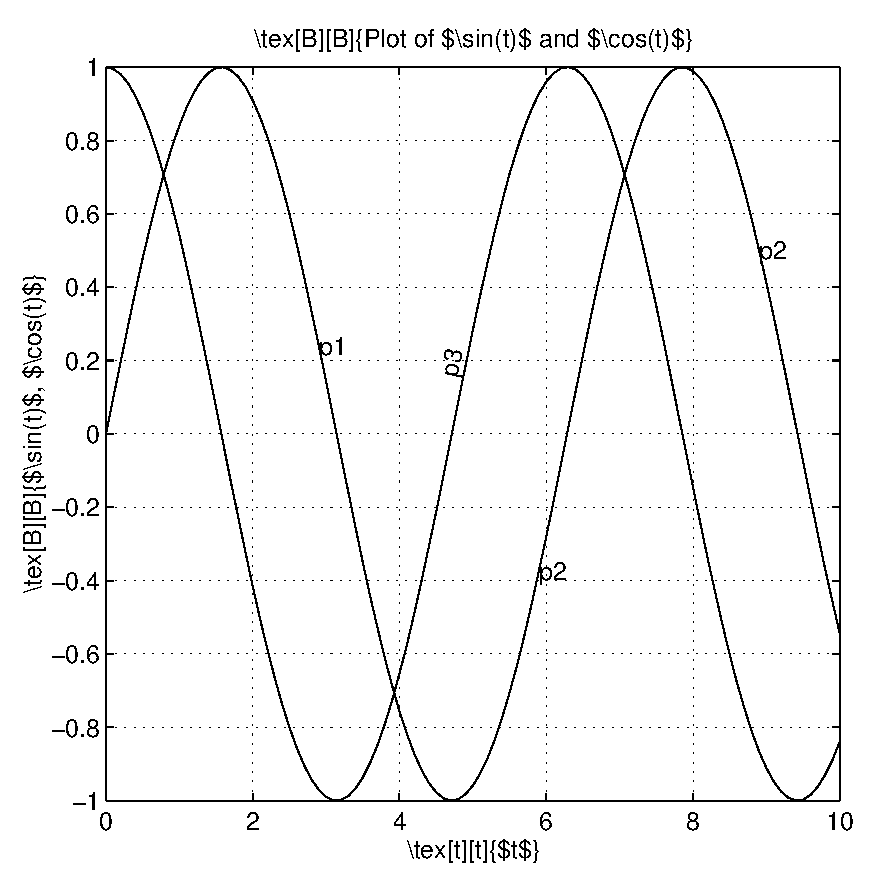
\includegraphics[width=3.5in]{example.eps}
         \end{center}
         \caption{A \textsf{psfrag} example.}
    \end{figure}
\end{verbatim}
Note the use of a |picture| environment within the replacement
for |p1|.

\begin{figure}[tbh]
    \unitlength=1in
    \begin{center}
        \psfragscanon
        \psfrag{p1}[l]{\begin{picture}(0,0)
            \put(0.15, 0.2){\makebox(0,0)[l]{$\sin(t)$}}
            \put(0.1,0.2){\vector(-1,-2){0.1}}
            \end{picture}}
        \psfrag*{p1}[][l]{$\ast$}
        \psfrag{p2}[][l]{$\ast$}
        \psfrag{p3}{$\cos(t)$}
        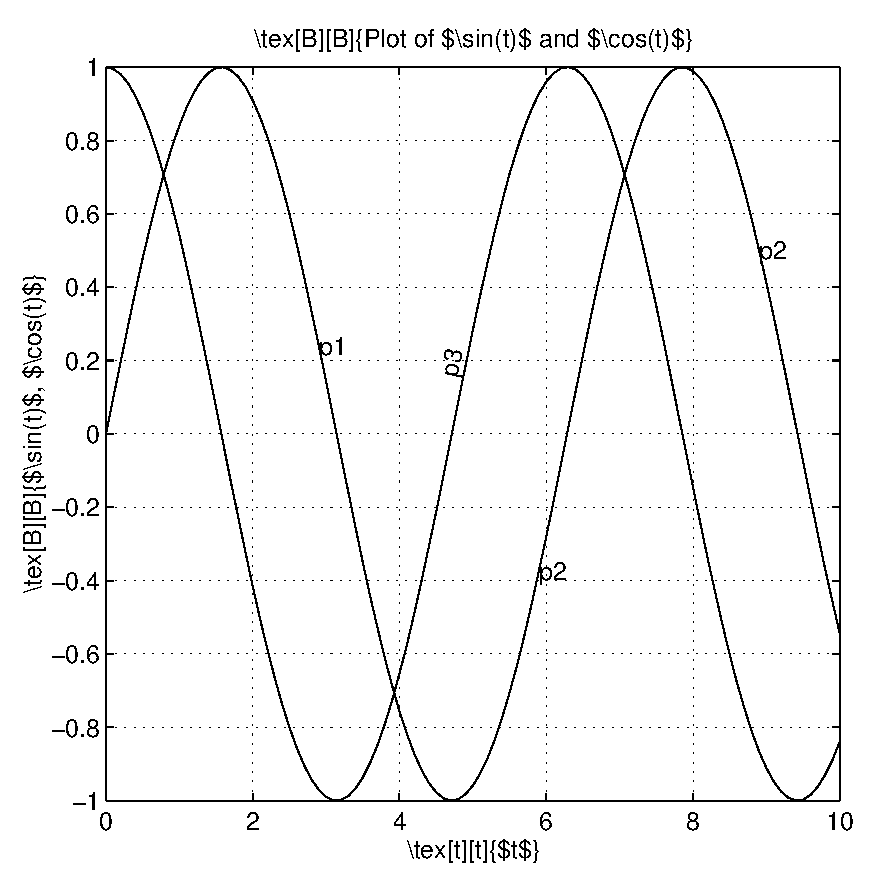
\includegraphics[width=3.5in]{example.eps}
   \end{center}
   \caption{A \pfg\ example.}
   \label{fig:example1}
\end{figure}
The result of these two steps is shown in Figure~\ref{fig:example1}.

\subsection{Figure scaling and resizing}
\label{sec:scaling}

There are two ways to resize EPS figures with the \pkg{graphics}
package, and each has as different effect on \pfg\ replacements. If you
are used to using \fname{epsf.sty}, you will be accustomed to only one
such behavior.

If you use the \cs{scalebox} or \cs{resizebox} macros of \fname{graphics.sty},
then the \pfg\ replacments \emph{will} scale with the figure. This
effect is illustrated in \ref{fig:example2} below.
\begin{figure}[tbh]\unitlength=1in
    \begin{center}
        \psfragscanon
        \psfrag{p1}[l]{\begin{picture}(0,0)
            \put(0.15, 0.2){\makebox(0,0)[l]{$\sin(t)$}}
            \put(0.1,0.2){\vector(-1,-2){0.1}}
            \end{picture}}
        \psfrag*{p1}[][l]{$\ast$}
        \psfrag{p2}[][l]{$\ast$}
        \psfrag{p3}{$\cos(t)$}
        \resizebox{3.5in}{!}{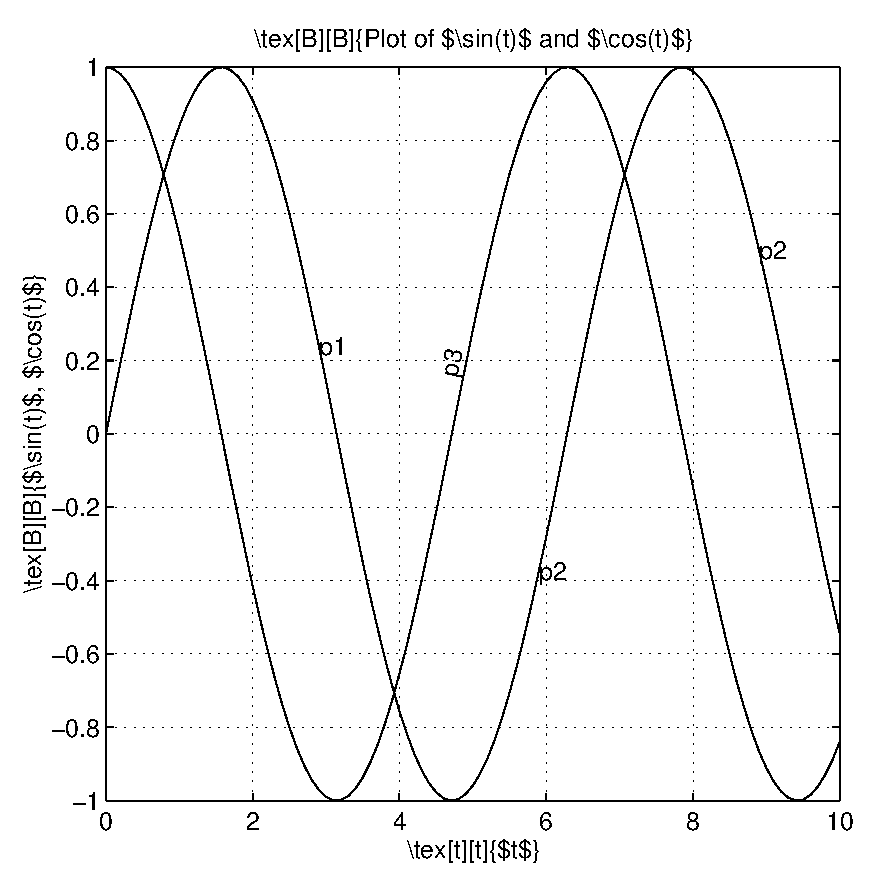
\includegraphics{example.eps}}
    \end{center}
    \caption{The same \pfg\ example as Figure~\ref{fig:example1}, using
             \cs{resizebox} to set the width.}
    \label{fig:example2}
\end{figure}
Figure~\ref{fig:example2} uses the following command to scale the figure
to 3.5 inches in width:
\begin{verbatim}
\resizebox{3.5in}{!}{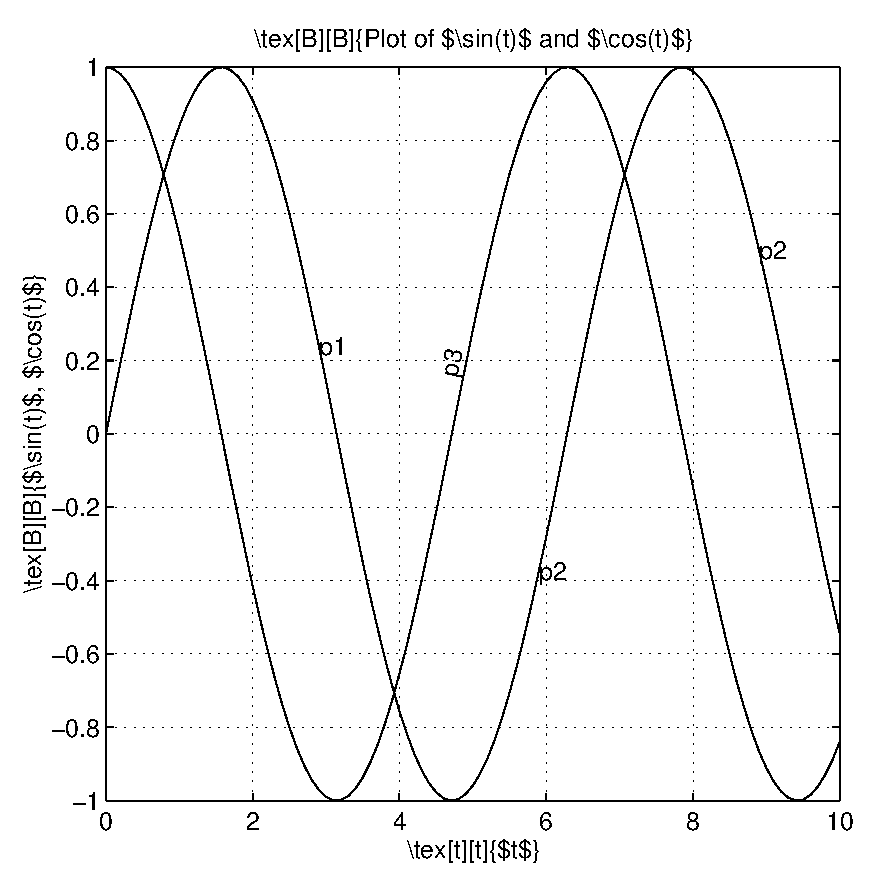
\includegraphics{example.eps}}
\end{verbatim} This
is in direct contrast to Figure~\ref{fig:example1}, which uses the
|width=| keyword from the \fname{graphicx.sty}, as follows:
\begin{verbatim}
\includegraphics[width=3.5in]{\includegraphics{example.eps}}
\end{verbatim}
Figure~\ref{fig:example1} also reflects the behavior that
you would see when using the \fname{epsf.sty} macros \cs{epfxsize},
\cs{epsfysize}, \emph{etc}. In these cases, the \pfg\ text does not
scale with it. to resize the figure.

As you can see, the text in the second figure is decidedly smaller
than the first. This is because \cs{resizebox} uses PostScript tricks to
scale \emph{all} of the contents of its argument. Since the \cs{psfrag}
commands are not actually typeset until \emph{within} the
\cs{includegraphics} command, they are resized as well.

The \fname{graphicx.sty} key-value pairs |width=|, |height=|,
and |scale=| scale the figure without scaling the replacement
text, as long as they are supplied \emph{before} an |angle=|
rotation key. Of course, the \cs{resizebox} and \cs{scalebox}
macros are still available in \fname{graphicx.sty}, so you can
mix and match both behaviors as you see fit. See the \pkg{graphics}
documentation for more details.

If you are still unsure about these distinctions, then try both
methods for scaling your figures until you find a convention that
works best for you.

\section{Common mistakes, known problems, and bugs}

\pfg\ is bug-free.

Well, of course we're kidding. \pfg\ uses some tricky PostScript hacks to
achieve its goals. So it really would not surprise us if you find bugs, If you
find any problems, please confirm they are not mentioned below; and, if not,
report them to te \pfg\ mailing list (see below).

\subsection{Using \pfg\ tags properly}
\label{sec:tags}

One of the more frequent problems that people encounter with \pfg\ is that it
replaces \emph{some} of their tags properly, but not all of them. Whenever
possible, you should design your figures \emph{with \pfg\ in mind}, by
following this rule:
\begin{quote}
	When adding a piece of text (a \emph{tag}) in a figure for \pfg\ to
	replace, use a \emph{single word}, containing only unaccented letters
	and numbers.	
\end{quote}
This is the way that \pfg\ is intended to be used; doing so will almost
guarantee that \pfg\ works as advertised. Of course, one cannot always follow
this rule; and a small handful of drawing packages consistently cause problems.
Invariably, these problems can be resolved by understanding how \pfg\ looks for
these tags.

PostScript has five commands to display text---|show|, |ashow|, |kshow|,
|widthshow|, and |awidthshow|---although, in many cases, an EPS file will
define abbreviations of these commands. \pfg\ actually \emph{intercepts} these
commands and checks them for the tags to replace. When the string matches a
known tag, \pfg\ figures out where the tag \emph{would} have been displayed,
and inserts its replacement there. When it doesn't, \pfg\ lets the |*show|
command proceed normally.

The strings that these |*show| display are delimited with parentheses, much
like the \fname{C} language uses double quotes. For example:
\begin{quote}
	|(This is a test.) show| ~~~~~~~~~~~~displays~~~~~~~~~~~~|This is a test.|
\end{quote}
Unmatched parentheses and
certain other special characters must be preceded by a backslash in a
PostScript string. For example:
\begin{quote}
	|(x = \(0,1]) show| ~~~~~~~~~~~~displays~~~~~~~~~~~~|x = (0,1]|
\end{quote}

With this in mind, here is the rule about \pfg\ tags:
\begin{quote}
	The tag supplied to the \cs{psfrag} command must be typed \emph{exactly
	as it appears in the EPS file's |*show| command}, without the surrounding
	parentheses.
\end{quote}
In other words, \pfg\ will work only if the string in the \cs{psfrag} command
exactly duplicates what is found in the EPS file. If your strings have
backslashes added to them, as in the |x = \(0,1]| example, then you will have
to add that backslash to the \cs{psfrag} command as well. And \pfg\ can only
replace \emph{entire} strings, not just parts of one. So if your EPS file
contains
\begin{quote}
	|(I want to replace the XXX here) show|
\end{quote}
then the \cs{psfrag} command will fail if you supply just the |XXX|.

You can use a simple text editor to check things, if you like; EPS files are
(almost always) just simple ASCII files.

Unfortunately, some drawing packages display text by sending each character
\emph{individually} to a |show| command. In other words, if you use the
drawing tool to put the string ``test'' in your figure, it will do something like this:
\begin{quote}
	|(t) show (e) show (s) show (t) show |
\end{quote}
If this is true in your case, we apologize; it makes using \pfg\ much more
inconvenient---you will be limited to single-character tags. Such tools
also prevent the use of the \cs{tex} command.

\subsection{Problems using some \pkg{xfig} figures}

\pfg\ does not work with \pkg{xfig} figures that use ``pattern fills.'' When
painting/filling a polygon, \pkg{xfig} provides a number of choices: simple
colors or grey levels, or a number of patterns like cross-hatches, checkers,
\etc\ Unfortunately, using a pattern fill in a figure processed by \pfg\ results
in PostScript files that will not print.

Fortunately, there are workarounds:
\begin{enumerate}
	\item Avoid pattern fills in your \pkg{xfig} figures; use simple
		  colors (or greys) instead. Consult the \pkg{xfig} documentation
		  for details.
	\item Open the offending \fname{.eps} file (generated by \pkg{fig2dev}
		  or \pkg{xfig}'s ``export'' command) with your favorite text editor.
		  Look for the definition \pscom{PATfill} command; inside this 
		  subroutine, replace \pscom{show} with \pscom{oldshow} (there is only
		  one occurrence).
\end{enumerate}
For those PostScript hackers out there: both \pfg\ and \pkg{xfig} redefine the
PostScript \pscom{show} command. \pscom{oldshow} is where \pkg{xfig} stores the
``old'' version of the command. If you can determine why this fix works, and
convince the \pkg{xfig} maintainers to make the change; or, if you can suggest
a fix for \pfg, please do.

\subsection{Problems using old versions of the \pkg{seminar} package}
\label{sec:sem-bug}

The popular \pkg{seminar} package was, for awhile, incompatbile with PSfrag
3.0. This is due to the fact that PSfrag relies on certain features of the
\LaTeXe\ output routine, while \pkg{seminar} still uses one largely borrowed
from \LaTeX\ 2.09.

The best solution for this problem is to make sure that you have the latest
version of the \pkg{seminar} package, which can be retrieved from any CTAN
site, likely from the same place you found \pfg. A web page for \pkg{seminar}
can be found at \fname{http://www.tug.org/applications/Seminar/}. The
1997/10/13 version seems to have corrected the problem.

If for some reason you are forced to use an older version, there is a
temporary, \pkg{dvips}-specific fix: add the command
|\special{header=psfrag.pro}| just before |\begin{document}| in your \LaTeX\
file.

\section{The \pfg\ mailing list}
\label{sec:mail}

There is a Majorodomo mailing list for purposes of \pfg\ maintenance.
It \emph{is not} intended to replace this manual or a small amount of
educated guesswork. But, it \emph{is} the perfect place for bug reports,
development ideas, and so forth. Anyone who wishes to assist in
\pfg's evolution may subscribe; to do so, just send mail to
\begin{quote}
 \netaddress{majordomo@rascals.stanford.edu}
\end{quote}
with the line |subscribe psfrag| in the \emph{body} of the text.

Bug supports, ideas, \emph{etc.} should go to
\begin{quote}
    \netaddress{psfrag@rascals.stanford.edu}.
\end{quote}
If you have found a bug to report, please provide us with the
necessary files (a \LaTeX\ file, the EPS figures, \etc) so we can
test it out ourselves! Try to provide us with the shortest
self-contained example that demonstrates your bug. If this is not
possible, drop us a line first.

\end{document}
